Leaflet adalah pustaka JavaScript open-source terkemuka untuk peta interaktif ramah-mobile. Dengan berat hanya sekitar 38 KB JS, ia memiliki semua fitur pemetaan yang paling dibutuhkan pengembang. Leaflet dirancang dengan kesederhanaan, kinerja, dan kegunaan dalam pikiran. Ini bekerja secara efisien di semua platform desktop dan seluler utama, dapat diperluas dengan banyak plugin, memiliki API yang indah, mudah digunakan dan didokumentasikan dengan baik dan kode sumber yang mudah dibaca dan menyenangkan untuk berkontribusi \cite{everviewleaflet}.


\section{Cara Menampilkan Map Leaflet JS di CodeIgniter}
\begin{enumerate}
    \item Buka salah satu file php yang ingin Anda berikan fitur map, file dapat ditemukan ada pada folder  \verb|C:/xampp7/htdocs/ci4_leafletjs/app/Views/|.
    \item Pada bagian \verb|<head>| sertakan file Leaflet CSS.
\begin{lstlisting}[caption=File Leaflet CSS]
<head>
    <meta charset="utf-8">
    <meta name="viewport" content="width=device-width, initial-scale=1.0, user-scalable=0, minimal-ui">
    <meta http-equiv="X-UA-Compatible" content="IE=edge" />
    <meta name="description" content="CodedThemes">
    <meta name="keywords" content=" Admin , Responsive, Landing, Bootstrap, App, Template, Mobile, iOS, Android, apple, creative app">
    <meta name="author" content="CodedThemes">
    
    <link rel="stylesheet" href="https://unpkg.com/leaflet@1.5.1/dist/leaflet.css"integrity="sha512-xwE/Az9zrjBIphAcBb3F6JVqxf46+CDLwfLMHloNu6KEQCAWi6HcDUbeOfBIptF7tcCzusKFjFw2yuvEpDL9wQ=="crossorigin=""/>
</head>
.....
\end{lstlisting}

    \item Kemudian sertakan file JavaScript Leaflet setelah CSS Leaflet, pada  bagian footer atau sebelum penutup \verb|</body>|.
\begin{lstlisting}[caption=File JavaScript Leaflet]
.....
    <script src="https://unpkg.com/leaflet@1.5.1/dist/leaflet.js"integrity="sha512-GffPMF3RvMeYyc1LWMHtK8EbPv0iNZ8/oTtHPx9/cc2ILxQ+u905qIwdpULaqDkyBKgOaB57QTMg7ztg8Jm2Og=="crossorigin=""></script>

</body>
</html>
\end{lstlisting}

    \item Map sudah siap untuk ditampilkan, selanjutnya adalah meletakkan elemen div dengan id tertentu di mana Anda ingin peta Anda berada.
\begin{lstlisting}[caption=Elemen div map Leaflet]
.....
    <div id="mapid"></div>
.....
\end{lstlisting}

    \item Jalankan aplikasi kemudian akan tampil map seperti berikut:
	\begin{figure}[!htbp]
		\centering
		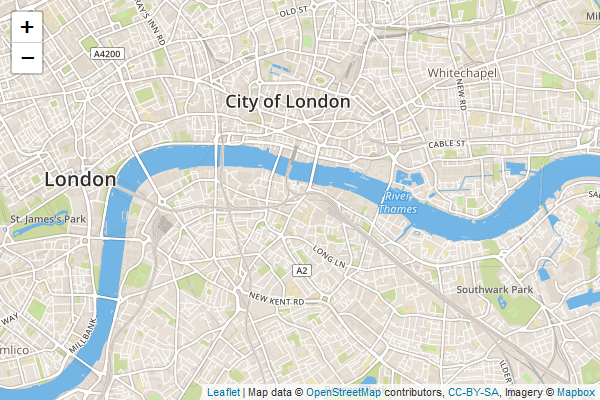
\includegraphics[width=0.5\textwidth]{figures/LEAFLETJS/LJS1.png}
		\label{Leaflet1}
	\end{figure}
\end{enumerate}





\section{Menampilkan Mapbox Pada index.php} 
\label{7.2}
Pada bab sebelumnya sudah dilakukan konfigurasi beberapa template untuk mepercantik tampilan index.php. Kemudian selanjutnya adalah bagaimana cara memasang mapbox pada index.php? Berikut caranya:
\begin{enumerate}
    \item Tambahkan config pada bagian head dan footer index.php dapat dilihat seperti pada codingan dibawah ini:

\begin{lstlisting}[caption=Menampilkan Mapbox Leaflet JS di CodeIgniter 4]
.....
<head>
    <link href="/algoritma/style/justified-nav.css" rel="stylesheet">
    <link href="https://fonts.googleapis.com/css?family=Open+Sans:400,600" rel="stylesheet">
    <link rel="stylesheet" href="https://unpkg.com/leaflet@1.3.1/dist/leaflet.css" integrity="sha512-Rksm5RenBEKSKFjgI3a41vrjkw4EVPlJ3+OiI65vTjIdo9brlAacEuKOiQ5OFh7cOI1bkDwLqdLw3Zg0cRJAAQ==" crossorigin=""/>
</head>
.....
  <script src="https://code.jquery.com/jquery-3.2.1.min.js"></script>
  <script src="https://cdnjs.cloudflare.com/ajax/libs/popper.js/1.11.0/umd/popper.min.js" integrity="sha384-b/U6ypiBEHpOf/4+1nzFpr53nxSS+GLCkfwBdFNTxtclqqenISfwAzpKaMNFNmj4" crossorigin="anonymous"></script>
  <script src="https://maxcdn.bootstrapcdn.com/bootstrap/4.0.0-beta/js/bootstrap.min.js" integrity="sha384-h0AbiXch4ZDo7tp9hKZ4TsHbi047NrKGLO3SEJAg45jXxnGIfYzk4Si90RDIq Nm1" crossorigin="anonymous"></script>
  <script src="https://cdn.jsdelivr.net/npm/d3@3.3.0/d3.min.js"></script>
  
  <script src="https://cdn.jsdelivr.net/npm/leaflet@0.7.7/dist/leaflet.js"></script>

  <script src="/algoritma/js/main.js"></script>
  <script src="/algoritma/js/ie10-viewport-bug-workaround.js"></script>
 .....
\end{lstlisting}

    \item Kemudian pada folder \verb|C:\xampp7\htdocs\ci4_leafletjs\public|, buat satu folder dengan nama algoritma dimana dalam folder ini akan di masukkan beberapa js tentang algoritma dijkstra dan floyd warshall dan js tentang package leaflet.
    \vspace{5cm}
	\begin{figure}[!htbp]
		\centering
		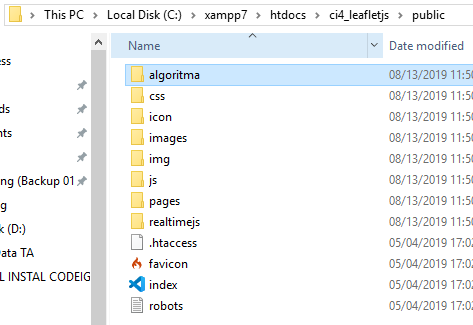
\includegraphics[width=0.5\textwidth]{figures/LEAFLETJS/LJS2.PNG}
		\label{Leaflet2}
	\end{figure}
	
	\item Buka folder algoritma kemudian buat folder dengan nama js dan buat file didalam folder js dengan nama main.js. Dalam file ini nantinya tersimpan beberapa konfigurasi seperti konfigurasi untuk leaflet js dan algoritma yang akan digunakan dalam penentuan rute terdekat.
	
	\item Buka file main.js kemudian isikan kodingan berikut:
\begin{lstlisting}[caption=Setting setView Pada Leaflet JS]
var graphmap, svg, maps, g;

var mapdata = {
    allnodes: [],
    paths: [],
    distances: [],
    getui: {
        htmlSelectStartingNode: "#from-starting",
        htmlSelectEndNode: "#to-end"
    },
    getstate: {
        selectedNode: null,
        fromNode: null,
        toNode: null
    }
};

maps = L.map('svg-map').setView([-6.8731953,107.5737873,17], 15);
//Menampilkan lokasi maps politeknik pos indonesia dengan max zoom 15 saat pertama kali load aplikasi
mapLink = '<a href="http://openstreetmap.org">OpenStreetMap</a>';
L.tileLayer('https://api.tiles.mapbox.com/v4/{id}/{z}/{x}/{y}.png?access_token={accessToken}', {
    attribution: 'Map data &copy; <a href="http://openstreetmap.org">OpenStreetMap</a> contributors, <a href="http://creativecommons.org/licenses/by-sa/2.0/">CC-BY-SA</a>, Imagery © <a href="http://mapbox.com">Mapbox</a>',
    maxZoom: 18,
    id: 'mapbox.streets',
    accessToken: 'pk.eyJ1IjoiaW1hZHVkZGluaGFyaXMiLCJhIjoiY2p1d2E3MzM4MGFiZDRkcGYyM WF3emtlYiJ9.KTemDE4IAujR0X-ltttotg'
}).addTo(maps);
maps._initPathRoot()
svg = d3.select("#svg-map").select("svg")
    .attr("class", "svgmap")
    .on("contextmenu", function () { d3.event.preventDefault(); })
\end{lstlisting}

    \item Simpan, kemudian panggil library js dalam index.php
\begin{lstlisting}[caption=Call Library setView]
<script src="/algoritma/js/main.js"></script>
\end{lstlisting}

    \item Berikut codingan full untuk tampilan index.php

\begin{lstlisting}[caption=Pemanggilan Library setView pada index.php]
<!DOCTYPE html>
<html lang="en">

<head>
    <meta charset="utf-8">
    <meta name="viewport" content="width=device-width, initial-scale=1.0, user-scalable=0, minimal-ui">
    <meta http-equiv="X-UA-Compatible" content="IE=edge" />
    <meta name="description" content="CodedThemes">
    <meta name="keywords" content=" Admin , Responsive, Landing, Bootstrap, App, Template, Mobile, iOS, Android, apple, creative app">
    <meta name="author" content="CodedThemes">
  <title>Shortest Path Algorithm</title>
  
  <link rel="stylesheet" href="https://maxcdn.bootstrapcdn.com/bootstrap/4.0.0-beta/css/bootstrap.min.css" integrity="sha384-/Y6pD6FV/Vv2HJnA6t+vslU6fwYXjCFtcEpHbNJ0lyAFsXTsjBbfaDjzALeQsN6M" crossorigin="anonymous">
  <link href="/algoritma/style/justified-nav.css" rel="stylesheet">
  
    <link rel="icon" type="image/png" href="/images/favicon-32x32.png" sizes="32x32" />
    <link rel="icon" type="image/png" href="/images/favicon-16x16.png" sizes="16x16" />
    <link rel="icon" href="/images/favicon.ico" type="image/x-icon">
    <link href="https://fonts.googleapis.com/css?family=Open+Sans:400,600" rel="stylesheet">
    <link rel="stylesheet" type="text/css" href="/css/bootstrap/css/bootstrap.min.css">
    <link rel="stylesheet" type="text/css" href="/icon/themify-icons/themify-icons.css">
    <link rel="stylesheet" type="text/css" href="/icon/icofont/css/icofont.css">
    <link rel="stylesheet" type="text/css" href="/css/datatables.css">
    <link rel="stylesheet" type="text/css" href="/css/buttons.dataTables.min.css">
    <link rel="stylesheet" type="text/css" href="/css/select2.css">
    <link rel="stylesheet" type="text/css" href="/css/style.css">
    <link rel="stylesheet" type="text/css" href="/css/style-bulog.css">
    <link rel="stylesheet" type="text/css" href="/css/style-bulog-print.css" media="print">
    <link rel="stylesheet" type="text/css" href="/css/jquery.mCustomScrollbar.css">
    <link rel="stylesheet" href="https://cdnjs.cloudflare.com/ajax/libs/font-awesome/4.7.0/css/font-awesome.min.css">

    <script type="text/javascript" src="/js/jquery/jquery.min.js"></script>
    <link rel="stylesheet" href="https://unpkg.com/leaflet@1.3.1/dist/leaflet.css" integrity="sha512-Rksm5RenBEKSKFjgI3a41vrjkw4EVPlJ3+OiI65vTjIdo9brlAacEuKOiQ5OFh7cOI1bkDwLqdLw3Zg0cRJAAQ==" crossorigin=""/>
</head>
<body>
    <div class="theme-loader">
      <div class="ball-scale">
        <img src="/images/logo-track.png"/>
      </div>
    </div>

    <div class="loading-wrap">
      <div class="loading-box">
        <img src="/images/logo-track.png"/>
        <span>Mohon tunggu...</span>
        <div class="progress" style="height: 10px;">
          <div id="progress-bar" class="progress-bar" role="progressbar"></div>
        </div>
      </div>
    </div>

    <div class="pcoded-content">
      <div class="pcoded-inner-content">
        <div class="main-body">
          <div class="page-wrapper">
            <div class="page-header card">
              <div class="row align-items-start">
                <div class="col-lg-12">
                  <div class="page-header-title">
                    <div class="icon-logo">
                      <img src="/images/logo-track.png"/>
                    </div>
                    <div class="d-inline">
                      <h4 class="m-b-15 block">Shortest Path Algorithm</h4>
                      <h3 class="m-t-5"><strong>Solusi Penentuan Jalur Terdekat</strong></h3>
                    </div>
                  </div>
                </div>
              </div>
            </div>
            <br />
          </div>
        </div>
      </div>
    </div>

    <div class="row">
      <div class="col-lg-12">
        <div id="svg-map" style="width: 1110px; height: 800px" class="card">
        </div>
      </div>
    </div>

    <div class="pcoded-content">
      <div class="pcoded-inner-content">
        <div class="main-body">
          <div class="page-wrapper">
            <div class="page-header card">
              <div class="row align-items-start">
                <div class="col-lg-8">
                  <div class="page-header-title">        
                    &copy; Faisal Syarifuddin <?php echo date('Y') ?>
                    <br>CodeIgniter Version <?= CodeIgniter\CodeIgniter::CI_VERSION ?>
                  </div>
                </div>
              </div>
            </div>
          </div>
        </div>
      </div>
    </div>
  </div>

  <script src="https://code.jquery.com/jquery-3.2.1.min.js"></script>
  <script src="https://cdnjs.cloudflare.com/ajax/libs/popper.js/1.11.0/umd/popper.min.js" integrity="sha384-b/U6ypiBEHpOf/4+1nzFpr53nxSS+GLCkfwBdFNTxtclqqenISfwAzpKaMNFNmj4" crossorigin="anonymous"></script>
  <script src="https://maxcdn.bootstrapcdn.com/bootstrap/4.0.0-beta/js/bootstrap.min.js" integrity="sha384-h0AbiXch4ZDo7tp9hKZ4TsHbi047NrKGLO3SEJAg45jXxnGIfYzk4Si90RDIq Nm1" crossorigin="anonymous"></script>
  <script src="https://cdn.jsdelivr.net/npm/d3@3.3.0/d3.min.js"></script>
  <script src="https://cdn.jsdelivr.net/npm/leaflet@0.7.7/dist/leaflet.js"></script>
  <script src="/algoritma/js/main.js"></script>
  <script src="/algoritma/js/ie10-viewport-bug-workaround.js"></script>
  <script type="text/javascript" src="/js/script.js"></script>

</body>
</html>
\end{lstlisting}

    \item Simpan file index.php tersebut kemudian jalankan aplikasi anda, maka pada browser aka muncup map box seperti pada gambar berikut.
	\begin{figure}[!htbp]
		\centering
		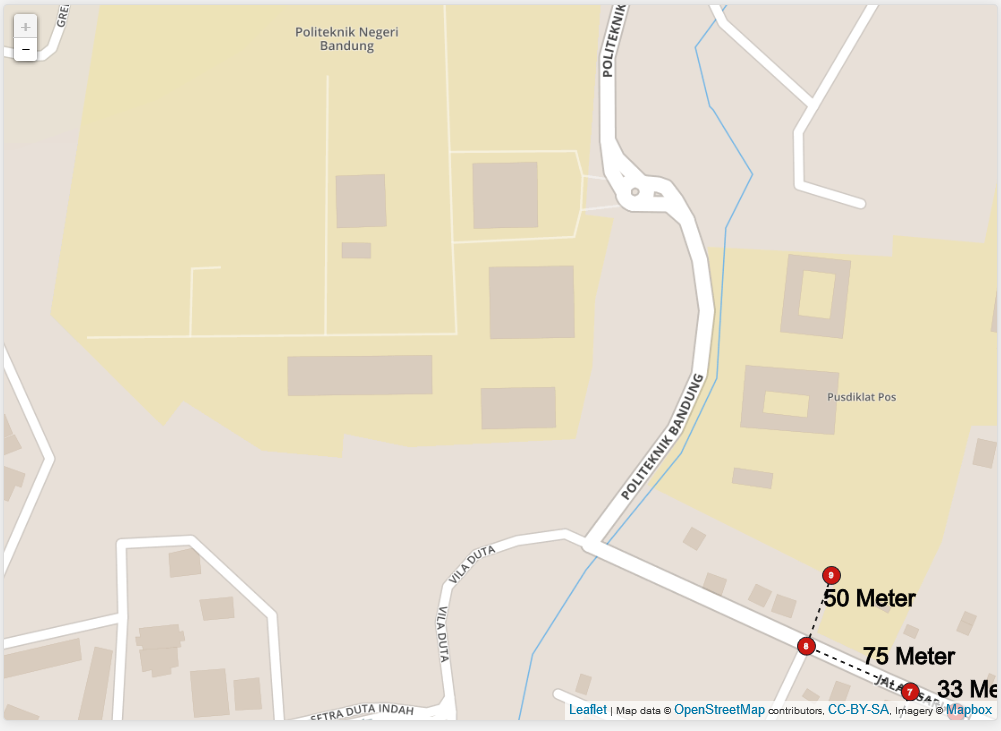
\includegraphics[width=0.5\textwidth]{figures/LEAFLETJS/LJS3.png}
		\label{Leaflet3}
	\end{figure}

\end{enumerate}




\section{Penetuan Jalur Terdekat Dengan Algoritma Dijkstra dan Floyd Warshal}
Melanjutnkan Kodingan sebelumnya, pada tahap ini anda akan membuat UI, dan beberapa function yang untuk algoritma dijsktra dan floyd warshal. Berikut tahapan membuat sistem penentuan jalur terdekat menggunakan algoritma dijsktra dan floyd warshall:
\begin{enumerate}
    \item Membuat index.php pada folder algoritma (Sebelumnya sudah di buat pada point \ref{7.2}).
    \item Melengkapi library yang ada pada index.php pada point \ref{7.2}, seperti pada kodingan dibawah:
\begin{lstlisting}[caption=index.php Full Code]
<!DOCTYPE html>
<html lang="en">

<head>
    <meta charset="utf-8">
    <meta name="viewport" content="width=device-width, initial-scale=1.0, user-scalable=0, minimal-ui">
    <meta http-equiv="X-UA-Compatible" content="IE=edge" />
    <meta name="description" content="CodedThemes">
    <meta name="keywords" content=" Admin , Responsive, Landing, Bootstrap, App, Template, Mobile, iOS, Android, apple, creative app">
    <meta name="author" content="CodedThemes">

  <title>Shortest Path Algorithm</title>
  <link rel="stylesheet" href="https://maxcdn.bootstrapcdn.com/bootstrap/4.0.0-beta/css/bootstrap.min.css" integrity="sha384-/Y6pD6FV/Vv2HJnA6t+vslU6fwYXjCFtcEpHbNJ0lyAFsXTsjBbfaDjzALeQsN6M" crossorigin="anonymous">
  <link href="/algoritma/style/justified-nav.css" rel="stylesheet">
  
    <link rel="icon" type="image/png" href="/images/favicon-32x32.png" sizes="32x32" />
    <link rel="icon" type="image/png" href="/images/favicon-16x16.png" sizes="16x16" />
    <link rel="icon" href="/images/favicon.ico" type="image/x-icon">
    <link href="https://fonts.googleapis.com/css?family=Open+Sans:400,600" rel="stylesheet">
    <link rel="stylesheet" type="text/css" href="/css/bootstrap/css/bootstrap.min.css">
    <link rel="stylesheet" type="text/css" href="/icon/themify-icons/themify-icons.css">
    <link rel="stylesheet" type="text/css" href="/icon/icofont/css/icofont.css">
    <link rel="stylesheet" type="text/css" href="/css/datatables.css">
    <link rel="stylesheet" type="text/css" href="/css/buttons.dataTables.min.css">
    <link rel="stylesheet" type="text/css" href="/css/select2.css">
    <link rel="stylesheet" type="text/css" href="/css/style.css">
    <link rel="stylesheet" type="text/css" href="/css/style-bulog.css">
    <link rel="stylesheet" type="text/css" href="/css/style-bulog-print.css" media="print">
    <link rel="stylesheet" type="text/css" href="/css/jquery.mCustomScrollbar.css">
    <link rel="stylesheet" href="https://cdnjs.cloudflare.com/ajax/libs/font-awesome/4.7.0/css/font-awesome.min.css">

    <script type="text/javascript" src="/js/jquery/jquery.min.js"></script>
    <link rel="stylesheet" href="https://unpkg.com/leaflet@1.3.1/dist/leaflet.css" integrity="sha512-Rksm5RenBEKSKFjgI3a41vrjkw4EVPlJ3+OiI65vTjIdo9brlAacEuKOiQ5OFh7cOI1bkDwLqdLw3Zg0cRJAAQ==" crossorigin=""/>

</head>
<body>
    <div class="theme-loader">
      <div class="ball-scale">
        <img src="/images/logo-track.png"/>
      </div>
    </div>

    <div class="loading-wrap">
      <div class="loading-box">
        <img src="/images/logo-track.png"/>
        <span>Mohon tunggu...</span>
        <div class="progress" style="height: 10px;">
          <div id="progress-bar" class="progress-bar" role="progressbar"></div>
        </div>
      </div>
    </div>

    <div class="pcoded-content">
      <div class="pcoded-inner-content">
        <div class="main-body">
          <div class="page-wrapper">
            <div class="page-header card">
              <div class="row align-items-start">
                <div class="col-lg-12">
                  <div class="page-header-title">
                    <div class="icon-logo">
                      <img src="/images/logo-track.png"/>
                    </div>
                    <div class="d-inline">
                      <h4 class="m-b-15 block">Shortest Path Algorithm</h4>
                      <h3 class="m-t-5"><strong>Solusi Penentuan Jalur Terdekat</strong></h3>
                    </div>
                  </div>
                </div>
              </div>
            </div>
            <br />
          </div>
        </div>
      </div>
    </div>

  <div class="container">
    <div class="row">
      <div class="col-lg-12">
            <label class="mr-sm-2" for="from">Cara penggunaan: Tentukan titik-titik sesuai di maps dengan cara klik kiri, kemudian sambungkan titik satu dengan titik lainnya dengan cara klik kanan titik awal dan klik kanan titik tujuan, pilih route dari mana kemana di pilihan titik awal dan titik tujuan kemudian klik start route untuk melihat hasil algoritma sesuai tombol yg diklik.</label>

        <hr>
          <div class="form-row align-items-center">
            <div class="col-auto">
              <label class="mr-sm-2" for="from">Titik Awal : </label>
              <select id="from-starting" class="custom-select mb-2 mr-sm-2 mb-sm-0"></select>
            </div>

            <div class="col-auto">
              <label class="mr-sm-2" for="to">Titik Tujuan : </label>
              <select id="to-end" class="custom-select mb-2 mr-sm-2 mb-sm-0"></select>
            </div>

            <div class="col-auto">
              <button type="button" id="getshortestroute" class="btn btn-primary" title="find shortest path between nodes using dijkstra"><i class="fa fa-map-o" aria-hidden="true"> Start Dijkstra</i></button>
            </div>
            
            <div class="col-auto">
              <button type="button" id="floyd" class="btn btn-primary" title="find shortest path between nodes using floyd"><i class="fa fa-map-o" aria-hidden="true"> Start Floyd</i></button>
            </div>

            <div class="col-auto">
              <button type="button" id="clearmap" class="btn btn-danger"><i class="fa fa-trash-o" aria-hidden="true"> Hapus Map</i></button>
            </div>

            <div class="col-12">
              <br><br>
              <h6>Jalur terpendek: <span id="jtp"></span></h6>
            </div>
          </div>

      </div>
    </div>

    <div class="row">
      <div class="col-lg-12">
        <div id="svg-map" style="width: 1110px; height: 800px" class="card">
        </div>
      </div>
    </div>

    <hr>
    <form style="margin-top:5px;">
    <div class="form-row align-items-center">
      <div class="col-auto">
        <button type="button" class="btn btn-primary" id="data-export"> Export Data</button>
      </div>
    </div>
    </form>
    <hr>
    
    <div class="col-auto" style="margin-top: 5px;">
      <label class="mr-sm-2" for="inlineFormCustomSelect">Route Wisata Bandung</label>
      <select class="custom-select mb-2 mr-sm-2 mb-sm-0" id="setexample">
        <option value="0"></option>
        <option value="1">Titik Wisata Bandung</option>
        <option value="2">Data Titik Lokasi Wisata Bandung</option>
        <option value="3">Sample Data Politeknik Pos Indonesia</option>
        <option value="4">Dusun Bambu Lembang</option>
        <option value="5">Farmhouse Lembang</option>
        <option value="6">Gunung Tangkuban Perhau</option>
        <option value="7">Kebun Teh Sukawana</option>
        <option value="9">Tebing Kraton</option>
        <option value="10">Alun-Alun Bandung</option>
      </select>
    </div>
    <hr>

    <div class="pcoded-content">
      <div class="pcoded-inner-content">
        <div class="main-body">
          <div class="page-wrapper">
            <div class="page-header card">
              <div class="row align-items-start">
                <div class="col-lg-8">
                  <div class="page-header-title">        
                    &copy; Faisal Syarifuddin <?php echo date('Y') ?>
                    <br>CodeIgniter Version <?= CodeIgniter\CodeIgniter::CI_VERSION ?>
                  </div>
                </div>
              </div>
            </div>
          </div>
        </div>
      </div>
    </div>

  </div>

  <script src="https://code.jquery.com/jquery-3.2.1.min.js"></script>
  <script src="https://cdnjs.cloudflare.com/ajax/libs/popper.js/1.11.0/umd/popper.min.js" integrity="sha384-b/U6ypiBEHpOf/4+1nzFpr53nxSS+GLCkfwBdFNTxtclqqenISfwAzpKaMNFNmj4" crossorigin="anonymous"></script>
  <script src="https://maxcdn.bootstrapcdn.com/bootstrap/4.0.0-beta/js/bootstrap.min.js" integrity="sha384-h0AbiXch4ZDo7tp9hKZ4TsHbi047NrKGLO3SEJAg45jXxnGIfYzk4Si90RDIqNm1" crossorigin="anonymous"></script>
  <script src="https://cdn.jsdelivr.net/npm/d3@3.3.0/d3.min.js"></script>
  <script src="https://cdn.jsdelivr.net/npm/leaflet@0.7.7/dist/leaflet.js"></script>

  <script src="/algoritma/js/main.js"></script>
  <script src="/algoritma/js/ie10-viewport-bug-workaround.js"></script>
  <script type="text/javascript" src="/js/script.js"></script>

</body>
</html>
\end{lstlisting}

    \item Selanjutnya membuat function algoritma Dijkstra dan Floyd Warshall
    \begin{enumerate}
        \item Function Algoritma Dijsktra
    \begin{enumerate}
        \item Buka file main.js yang sudah dibuat sebelumnya pada point \ref{7.2} atau bisa ditemukan pada folder \verb|ci4_leafletjs\| kemudian dalam folder \verb|public\algoritma\js\main.js|.
        % C:\xampp7\htdocs\
        \item Buat functioin klik dijsktra pada main.js
\begin{lstlisting}[caption=Function OnClick Dijsktra]
$('#getshortestroute').on('click', function () {
    alert('Dijkstra');
    d3.selectAll("line").classed({ "shortest": false });
    calculateDistancesbetweennodes();
    if (!$(mapdata.getui.htmlSelectStartingNode).val() || !$(mapdata.getui.htmlSelectEndNode).val()) return;
    var sourceNode = $(mapdata.getui.htmlSelectStartingNode).val();
    var targetNode = $(mapdata.getui.htmlSelectEndNode).val();
    var results = dijkstra(sourceNode, targetNode);
    var distTotal = 0;
    var dist = null;
    var stepnode = '';
    if (results.path) {
        results.path.forEach(function (step) {

            dist = mapdata.distances[step.source][step.target]
            stepLine = d3.select(
                "line.from" + step.source + "to" + step.target + ","
                + "line.from" + step.target + "to" + step.source
            );
            stepLine.classed({ "shortest": true });
            stepnode += step.source+'->'+step.target+'->';
            distTotal = distTotal + dist;
        });
            var estimasiMenit = distTotal / 60; //perkiraan kecepatan 60 km/jam
            // var estimasiDetik = estimasiMenit * 3600 / 60;
            // var estimasiDetik = estimasiMenit * 60 / 3600;
            var estimasiDetik = (estimasiMenit - Math.floor(estimasiMenit)) * 60;
            var persentasilocaccuarcy = distTotal / 400;
                if(persentasilocaccuarcy <= 800){
                    persentasiloc = 'High';
                }else if(persentasilocaccuarcy >= 5000){
                    persentasiloc = 'Low';
                }else{
                    persentasiloc = 'Medium';
                }
            $('#jtp').html('(Dijkstra) '+Math.round(distTotal)+' m <br><br>Melewati node : start->'+stepnode+'end<br><br>Perkiraan waktu perjalanan: '+Math.round(estimasiMenit)+' menit, '+Math.round(estimasiDetik)+'detik<br><br>Persentasi Akurasi: '+persentasiloc+' ('+Math.round(persentasilocaccuarcy)+' %)');
    }

});
$('#clearmap').on('click', function () {
    clearGraph();
});
\end{lstlisting}
\label{FunctionOnClickDijsktra}
    \item Function ini akan di eksekusi ketika button pada index.php dengan id=getshortestroute di klik (button dijsktra).
\begin{lstlisting}[caption=Button Dijsktra]
<button type="button" id="getshortestroute" class="btn btn-primary" title="find shortest path between nodes using dijkstra">
\end{lstlisting}
\label{ButtonDijsktra}

    \item Selanjutnya membuat function dengan rumus dijsktra yang dihasilkan dari code listing psoudocode \ref{PseudocodeAlgoritmaDijkstra}. Function ini akan digunakan untuk mengeksekusi beberapa titik yang digunakan untuk menentukan jalur terdekat.
\begin{lstlisting}[caption=Function Algoritma Dijsktra]
function dijkstra(start, end) {
    var nodeCount = mapdata.distances.length,
        infinity = 99999, // infinity
        shortestPath = new Array(nodeCount),
        nodeChecked = new Array(nodeCount),
        pred = new Array(nodeCount);

    for (var i = 0; i < nodeCount; i++) {
        shortestPath[i] = infinity;
        pred[i] = null;
        nodeChecked[i] = false;
    }

    shortestPath[start] = 0;
    for (var i = 0; i < nodeCount; i++) {
        var minDist = infinity;
        var closestNode = null;
        for (var j = 0; j < nodeCount; j++) {
            if (!nodeChecked[j]) {
                if (shortestPath[j] <= minDist) {
                    minDist = shortestPath[j];
                    closestNode = j;
                }
            }
        }

        nodeChecked[closestNode] = true;
        for (var k = 0; k < nodeCount; k++) {
            if (!nodeChecked[k]) {
                var nextDistance = distanceBetween(closestNode, k, mapdata.distances);
                if ((parseInt(shortestPath[closestNode]) + parseInt(nextDistance)) < parseInt(shortestPath[k])) {
                    soFar = parseInt(shortestPath[closestNode]);
                    extra = parseInt(nextDistance);
                    shortestPath[k] = soFar + extra;
                    pred[k] = closestNode;
                }
            }
        }
    }

    if (shortestPath[end] < infinity) {
        var newPath = [];
        var step = {
            target: parseInt(end)
        };
        var v = parseInt(end);

        while (v >= 0) {
            v = pred[v];
            if (v !== null && v >= 0) {
                step.source = v;
                newPath.unshift(step);
                step = {
                    target: v
                };
            }
        }

        totalDistance = shortestPath[end];
        return {
            mesg: 'Status: OK',
            path: newPath,
            source: start,
            target: end,
            distance: totalDistance
        };
    } else {
        return {
            mesg: 'Sorry No path found',
            path: null,
            source: start,
            target: end,
            distance: 0
        };
    }

    function distanceBetween(fromNode, toNode, distances) {
        dist = distances[fromNode][toNode];
        if (dist === 'x') dist = infinity;
        return dist;
    }
};
\end{lstlisting}
\par Function ini akan di eksekusi ketika button dijsktra diklik, kemudian akan memanggil function dijsktra pada variable "var results = dijkstra(sourceNode, targetNode);" di function onclick button dijkstra.
    \end{enumerate}
    
    \item Function Algoritma Floyd Warshall
    \begin{enumerate}
        \item Masih di file main.js, buat functioin klik floyd warshal pada main.js
\begin{lstlisting}[caption=Function OnClick Dijsktra]
$('#floyd').on('click', function () {
    alert('Floyd Warshal');
    d3.selectAll("line").classed({ "shortest": false });
    calculateDistancesbetweennodes();
    if (!$(mapdata.getui.htmlSelectStartingNode).val() || !$(mapdata.getui.htmlSelectEndNode).val()) return;
    var sourceNode = $(mapdata.getui.htmlSelectStartingNode).val();
    var targetNode = $(mapdata.getui.htmlSelectEndNode).val();
    var results = floyd(sourceNode, targetNode);
    var distTotal = 0;
    var dist = null;
    var stepnode = '';
    
    if (results.path) {
        results.path.forEach(function (step) {

            dist = mapdata.distances[step.source][step.target]
            stepLine = d3.select(
                "line.from" + step.source + "to" + step.target + ","
                + "line.from" + step.target + "to" + step.source
            );
            stepLine.classed({ "shortest": true });
            stepnode += step.source+'->'+step.target+'->';
            distTotal = distTotal + dist;
        });
            var estimasiMenit = distTotal / 60; //perkiraan kecepatan 60 km/jam
            var estimasiDetik = (estimasiMenit - Math.floor(estimasiMenit)) * 60;
            var persentasilocaccuarcy = distTotal / 400;
                if(persentasilocaccuarcy <= 800){
                    persentasiloc = 'High';
                }else if(persentasilocaccuarcy >= 5000){
                    persentasiloc = 'Low';
                }else{
                    persentasiloc = 'Medium';
                }
            $('#jtp').html('(Floyd Warshall) '+Math.round(distTotal)+' m <br><br>Melewati node : start->'+stepnode+'end<br><br>Perkiraan waktu perjalanan: '+Math.round(estimasiMenit)+' menit, '+Math.round(estimasiDetik)+'detik<br><br>Persentasi Akurasi: '+persentasiloc+' ('+Math.round(persentasilocaccuarcy)+' %)');
    }else{
        results.path.forEach(function (step) {

            dist = mapdata.distances[step.source][step.target]
            stepLine = d3.select(
                "line.from" + step.source + "to" + step.target + ","
                + "line.from" + step.target + "to" + step.source
            );
            stepLine.classed({ "shortest": true });
            stepnode += step.source+'->'+step.target+'->';
            distTotal = distTotal + dist;
        });
            var estimasiMenit = distTotal / 60; //perkiraan kecepatan 60 km/jam
            var estimasiDetik = (estimasiMenit - Math.floor(estimasiMenit)) * 60;
            var persentasilocaccuarcy = distTotal / 400;
                if(persentasilocaccuarcy <= 800){
                    persentasiloc = 'High';
                }else if(persentasilocaccuarcy >= 5000){
                    persentasiloc = 'Low';
                }else{
                    persentasiloc = 'Medium';
                }
            $('#jtp').html(Math.round(distTotal)+' m <br><br>Melewati node : start->'+stepnode+'end<br><br>Perkiraan waktu perjalanan: '+Math.round(estimasiMenit)+' menit, '+Math.round(estimasiDetik)+'detik<br><br>Persentasi Akurasi: '+persentasiloc+' ('+Math.round(persentasilocaccuarcy)+' %)');
    }

});
$('#clearmap').on('click', function () {
    clearGraph();
});
\end{lstlisting}

    \item Function ini akan di eksekusi ketika button pada index.php dengan id=floyd di klik (button dijsktra)
\begin{lstlisting}[caption=Button Dijsktra]
<button type="button" id="floyd" class="btn btn-primary" title="find shortest path between nodes using floyd"><i class="fa fa-map-o" aria-hidden="true"> Start Floyd</i></button>
\end{lstlisting}

    \item Selanjutnya membuat function dengan rumus floyd warshal yang dihasilkan dari code listing psoudocode \ref{PseudocodeAlgoritmaFloydWarshall}. Function ini akan digunakan untuk mengeksekusi beberapa titik yang digunakan untuk menentukan jalur terdekat.
    
\begin{lstlisting}[caption=Function Algoritma Dijsktra]
function floyd(start,end){
    console.log('start: '+start);
    console.log('end: '+end);
    var nodeCount = mapdata.distances.length,
        infinity = 99999, // infinity
        shortestPath = new Array(nodeCount),
        nodeChecked = new Array(nodeCount),
        pred = new Array(nodeCount);
        console.log('nodecount: '+nodeCount);

    for (var i = 0; i < nodeCount; i++) {
        shortestPath[i] = infinity;
        pred[i] = null;
        nodeChecked[i] = false;
    }
    shortestPath[start] = 0;

    for (var i = 0; i < nodeCount; i++) {
        var minDist = infinity;
        var closestNode = null;
        for (var j = 0; j < nodeCount; j++) {
            if (!nodeChecked[j]) {
                if (shortestPath[j] <= minDist) {
                    minDist = shortestPath[j];
                    closestNode = j;
                }
            }
        }
        nodeChecked[closestNode] = true;
        
        if(start>end){
            for (var k = closestNode; k > 0; k--) {
                if (!nodeChecked[k]) {
                    var nextDistance = distanceBetween(closestNode, k, mapdata.distances);
                    if ((parseInt(shortestPath[closestNode]) + parseInt(nextDistance)) < parseInt(shortestPath[k])) {
                        soFar = parseInt(shortestPath[closestNode]);
                        extra = parseInt(nextDistance);
                        shortestPath[k] = soFar + extra;
                        pred[k] = closestNode;
                    }
                }
            }
        }else{
            for (var k = closestNode; k < nodeCount; k++) {
                if (!nodeChecked[k]) {
                    var nextDistance = distanceBetween(closestNode, k, mapdata.distances);
                    if ((parseInt(shortestPath[closestNode]) + parseInt(nextDistance)) < parseInt(shortestPath[k])) {
                        soFar = parseInt(shortestPath[closestNode]);
                        extra = parseInt(nextDistance);
                        shortestPath[k] = soFar + extra;
                        pred[k] = closestNode;
                    }
                }
            }
        }
    }
    console.log('shortestPath[end]: '+shortestPath[end]);
    if (shortestPath[end] < infinity) {
        var newPath = [];
        var step = {
            target: parseInt(end)
        };

        var v = parseInt(end);
        while (v >= 0) {
            v = pred[v];
            if (v !== null && v >= 0) {
                step.source = v;
                newPath.unshift(step);
                step = {
                    target: v
                };
            }
        }
        totalDistance = shortestPath[end];

        return {
            mesg: 'Status: OK',
            path: newPath,
            source: start,
            target: end,
            distance: totalDistance
        };
    } else {
        return {
            mesg: 'Sorry No path found',
            path: null,
            source: start,
            target: end,
            distance: 0
        };
    }

    function distanceBetween(fromNode, toNode, distances) {
        dist = distances[fromNode][toNode];
        if (dist === 'x') dist = infinity;
        return dist;
    }
}
\end{lstlisting}
\par Function ini akan di eksekusi ketika button floyd warshall diklik, kemudian akan memanggil function floyd pada variable "var results = floyd(sourceNode, targetNode);" di function onclick button dijkstra.
    \end{enumerate}
    \end{enumerate}
    
    \item Membuat function penanda saat klik maps, ketika melakukan pemilihan lokasi maka mark yang akan muncul pada maps adalah mark dengan bentuk circle merah, berikut kodingan function:
\begin{lstlisting}[caption=Function Mark Maps]
function redrawNodes() {
    svg.selectAll("g.nodes").data([]).exit().remove();
    var elements = svg.selectAll("g.nodes").data(mapdata.allnodes, function (d, i) { return d.name; });
    var nodesEnter = elements.enter().append("g")
        .attr("class", "nodes");

    elements.attr("transform", function (d, i) {
        return "translate(" +
            maps.latLngToLayerPoint(new L.LatLng(d.x, d.y)).x + "," +
            maps.latLngToLayerPoint(new L.LatLng(d.x, d.y)).y + ")";
    });

    nodesEnter.append("circle")
        .attr("nodeId", function (d, i) { return i; })
        .attr("r", '20')
        .attr("class", "node")
        .style("cursor", "pointer")
        .on('click', nodeClick)
        .on("mouseenter", function () { maps.dragging.disable(); })
        .on("mouseout", function () { maps.dragging.enable(); })
        .on('contextmenu', function (d, i) { startEndPath(i); })
        .call(dragManager)

    nodesEnter
        .append("text")
        .attr("nodeLabelId", function (d, i) { return i; })
        .attr("dx", "-3")
        .attr("dy", "3")
        .attr("class", "label")
        .on('contextmenu', function (d, i) { startEndPath(i); })
        .call(dragManager)
        .text(function (d, i) { return d.name });
    elements.exit().remove();
};
\end{lstlisting}

    \item Membuat item line, penghubung antara titik satu dengan titik lainnya, fungsi ini akan menghubungkan node marks maps yang kemudian di eksekusi pada masing algoritma.
\begin{lstlisting}[caption=Function Lines Maps]
function redrawLines() {
    svg.selectAll("g.line").data([]).exit().remove();
    var elements = svg
        .selectAll("g.line")
        .data(mapdata.paths, function (d) { return d.id });
    var newElements = elements.enter();

    var group = newElements
        .append("g")
        .attr("class", "line");

    var line = group.append("line")
        .attr("class", function (d) {
            return "from" + mapdata.allnodes[d.from].name + "to" + mapdata.allnodes[d.to].name
        })
        .attr("x1", function (d) { return maps.latLngToLayerPoint(new L.LatLng(mapdata.allnodes[d.from].x, mapdata.allnodes[d.from].y)).x; })
        .attr("y1", function (d) { return maps.latLngToLayerPoint(new L.LatLng(mapdata.allnodes[d.from].x, mapdata.allnodes[d.from].y)).y; })
        .attr("x2", function (d) { return maps.latLngToLayerPoint(new L.LatLng(mapdata.allnodes[d.to].x, mapdata.allnodes[d.to].y)).x; })
        .attr("y2", function (d) { return maps.latLngToLayerPoint(new L.LatLng(mapdata.allnodes[d.to].x, mapdata.allnodes[d.to].y)).y; });

    var text = group.append("text")
        .attr("x", function (d) { return parseInt((maps.latLngToLayerPoint(new L.LatLng(mapdata.allnodes[d.from].x, mapdata.allnodes[d.from].y)).x + maps.latLngToLayerPoint(new L.LatLng(mapdata.allnodes[d.to].x, mapdata.allnodes[d.to].y)).x) / 2) + 5; })
        .attr("y", function (d) { return parseInt((maps.latLngToLayerPoint(new L.LatLng(mapdata.allnodes[d.from].x, mapdata.allnodes[d.from].y)).y + maps.latLngToLayerPoint(new L.LatLng(mapdata.allnodes[d.to].x, mapdata.allnodes[d.to].y)).y) / 2) - 5; })
        .attr("class", "line-label");

    elements.selectAll("text")
        .text(function (d) {
            return Math.round(mapdata.distances[d.from][d.to]) + " Meter";
        });
    elements.exit().remove();
};
\end{lstlisting}

    \item Save semua function yang dibuat dan jalankan aplikasi dengan cara buka terminal pada visual studio code kemudian masuk ke folder public dan masukkan perintah php -S localhost:8080.
	\begin{figure}[!htbp]
		\centering
		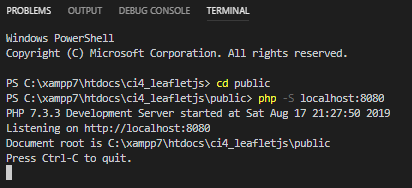
\includegraphics[width=0.5\textwidth]{figures/CODEIGNITER4/CI8.PNG}
	\end{figure}
	
	\vspace{4cm}
	\item Jalankan aplikasi \verb|ci4_leafletjs| anda pada browser kesayangan anda, dengan cara mengetikkan "localhost:8080", maka akan muncul tampilan seperti berikut:
	\begin{figure}[!htbp]
		\centering
		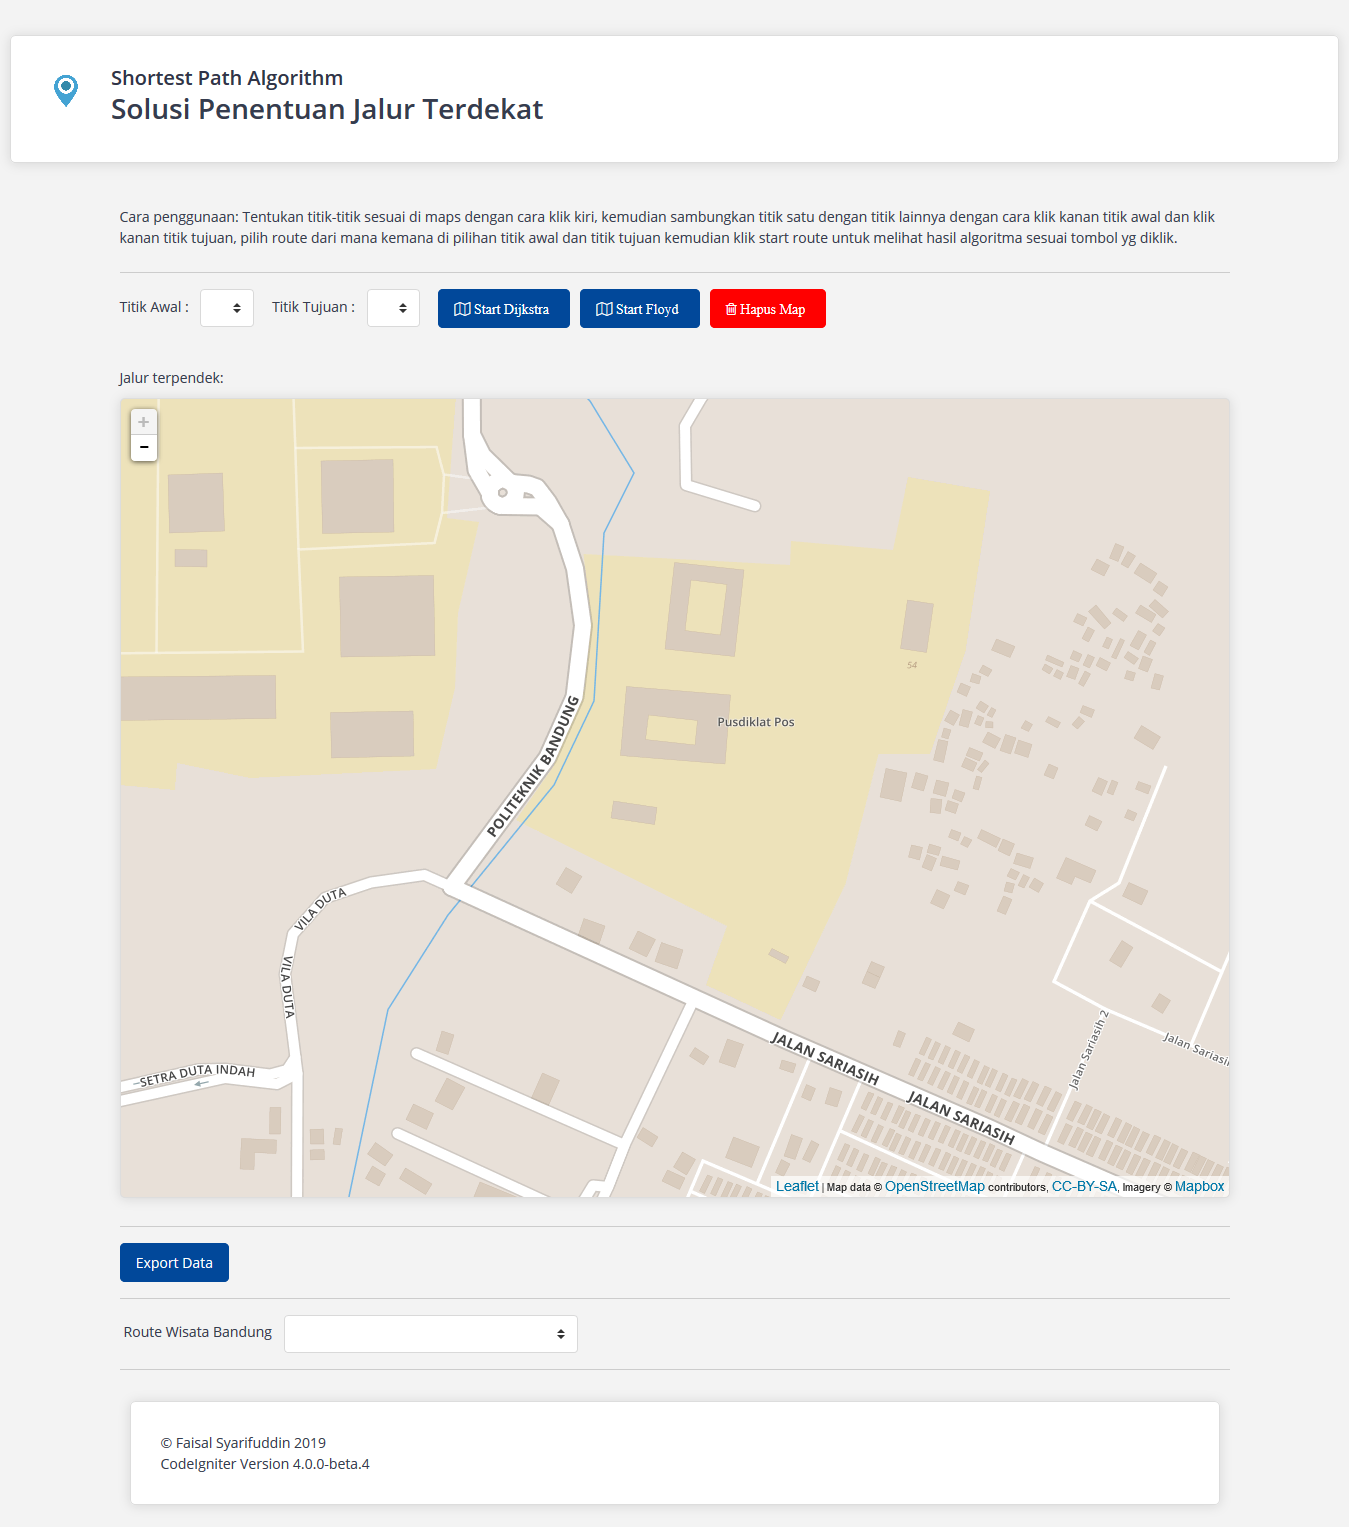
\includegraphics[width=0.5\textwidth]{figures/LEAFLETJS/LJS4.png}
		\label{Leaflet4}
	\end{figure}
	
\end{enumerate}